\documentclass[1pt]{book}



%%%%%%%%%%%%%%Include Packages%%%%%%%%%%%%%%%%%%%%%%%%%%
\usepackage{xcolor}
\usepackage{mathtools}
\usepackage[legalpaper, margin=1in]{geometry}
\usepackage{amsmath}
\usepackage{amssymb}
\usepackage{paralist}
\usepackage{rsfso}
\usepackage{amsthm}
\usepackage{wasysym}
\usepackage[inline]{enumitem}   
\usepackage{hyperref}
\usepackage{tocloft}
\usepackage{wrapfig}
\usepackage{titlesec}
\usepackage{colortbl}
\usepackage{stackengine} 
%%%%%%%%%%%%%%%%%%%%%%%%%%%%%%%%%%%%%%%%%%%%%%%%%%%%%%%%


%%%%%%%%%%%%%%%Chapter Setting%%%%%%%%%%%%%%%%%%%%%%%%%%
\definecolor{gray75}{gray}{0.75}
\newcommand{\hsp}{\hspace{20pt}}
\titleformat{\chapter}[hang]{\Huge\bfseries}{\thechapter\hsp\textcolor{gray75}{$\mid$}\hsp}{0pt}{\Huge\bfseries}
%%%%%%%%%%%%%%%%%%%%%%%%%%%%%%%%%%%%%%%%%%%%%%%%%%%%%%%%

%%%%%%%%%%%%%%%%%Theorem environments%%%%%%%%%%%%%%%%%%%
\newtheoremstyle{break}
  {\topsep}{\topsep}%
  {\itshape}{}%
  {\bfseries}{}%
  {\newline}{}%
\theoremstyle{break}
\theoremstyle{break}
\newtheorem{axiom}{Axiom}
\newtheorem{thm}{Theorem}[section]
\renewcommand{\thethm}{\arabic{section}.\arabic{thm}}
\newtheorem{lem}{Lemma}[thm]
\newtheorem{prop}[lem]{Proposition}
\newtheorem{corL}{Corollary}[lem]
\newtheorem{corT}[lem]{Corollary}
\newtheorem{defn}{Definition}[corL]
\newenvironment{indEnv}[1][Proof]
  {\proof[#1]\leftskip=1cm\rightskip=1cm}
  {\endproof}
%%%%%%%%%%%%%%%%%%%%%%%%%%%%%%%%%%%%%%%%%%%%%%%%%%%%%%

%%%%%%%%%%%%%%%%%%%%%%%Integral%%%%%%%%%%%%%%%%%%%%%%%
\def\upint{\mathchoice%
    {\mkern13mu\overline{\vphantom{\intop}\mkern7mu}\mkern-20mu}%
    {\mkern7mu\overline{\vphantom{\intop}\mkern7mu}\mkern-14mu}%
    {\mkern7mu\overline{\vphantom{\intop}\mkern7mu}\mkern-14mu}%
    {\mkern7mu\overline{\vphantom{\intop}\mkern7mu}\mkern-14mu}%
  \int}
\def\lowint{\mkern3mu\underline{\vphantom{\intop}\mkern7mu}\mkern-10mu\int}
%%%%%%%%%%%%%%%%%%%%%%%%%%%%%%%%%%%%%%%%%%%%%%%%%%%%%%



\newcommand{\R}{\mathbb{R}}
\newcommand{\N}{\mathbb{N}}
\newcommand{\Z}{\mathbb{Z}}
\newcommand{\Q}{\mathbb{Q}}
\newcommand{\D}{\mathcal{D}}
\newcommand{\J}{\mathcal{J}}
\newcommand{\T}{\mathcal{T}}
\newcommand{\Td}{\mathcal{T}_d}
\newcommand{\C}{\mathcal{C}}
\newcommand{\M}{\mathcal{M}}
\newcommand{\Lt}{\mathcal{L}}
\newcommand{\Symm}{\text{Symm}}
\newcommand{\A}{\mathcal{A}}
\newcommand{\Alt}{\text{Alt}}
\newcommand{\Int}{\text{Int}}
\newcommand{\Bd}{\text{Bd}}
\newcommand{\Complex}{\mathbb{C}}
\newcommand{\Power}{\mathcal{P}}
\newcommand{\ee}{\cdot 10}
\newcommand{\spa}{\text{span}}
\newcommand{\supp}{\text{supp}}
\newcommand{\sgn}{\text{sgn}}
\newcommand{\degr}{\text{deg}}
\newcommand{\Ecm}{\text{Ecm}}
\newcommand{\pd}{\partial}
\newcommand{\that}[1]{\widetilde{#1}}
\newcommand{\lr}[1]{\left(#1\right)}
\newcommand{\vmat}[1]{\begin{vmatrix} #1 \end{vmatrix}}
\newcommand{\bmat}[1]{\begin{bmatrix} #1 \end{bmatrix}}
\newcommand{\pmat}[1]{\begin{pmatrix} #1 \end{pmatrix}}
\newcommand{\rref}{\xrightarrow{\text{row\ reduce}}}
\newcommand{\txtarrow}[1]{\xrightarrow{\text{#1}}}
\newcommand\oast{\stackMath\mathbin{\stackinset{c}{0ex}{c}{0ex}{\ast}{\Circle}}}


\newcommand{\note}{\color{red}Note: \color{black}}
\newcommand{\remark}{\color{blue}Remark: \color{black}}
\newcommand{\example}{\color{green}Example: \color{black}}
\newcommand{\exercise}{\color{green}Exercise: \color{black}}

%%%%%%%%%%%%%%%%%%%%%%Roman Number%%%%%%%%%%%%%%%%%%%%%%%
\makeatletter
\newcommand*{\rom}[1]{\expandafter\@slowromancap\romannumeral #1@}
\makeatother
%%%%%%%%%%%%%%%%%%%%%%%%%%%%%%%%%%%%%%%%%%%%%%%%%%%%%%%%%

%%%%%%%%%%%%table of contents%%%%%%%%%%%%%%%%%%%%%%%%%%%%
\setlength{\cftchapindent}{0em}
\cftsetindents{section}{2em}{3em}

\renewcommand\cfttoctitlefont{\hfill\huge\bfseries}
\renewcommand\cftaftertoctitle{\hfill\mbox{}}

\setcounter{tocdepth}{2}
%%%%%%%%%%%%%%%%%%%%%%%%%%%%%%%%%%%%%%%%%%%%%%%%%%%%%%%%%


%%%%%%%%%%%%%%%%%%%%%Footnotes%%%%%%%%%%%%%%%%%%%%%%%%%%%
\newcommand\blfootnote[1]{%
  \begingroup
  \renewcommand\thefootnote{}\footnote{#1}%
  \addtocounter{footnote}{-1}%
  \endgroup
}
%%%%%%%%%%%%%%%%%%%%%%%%%%%%%%%%%%%%%%%%%%%%%%%%%%%%%%%%%

\makeatletter
\def\@seccntformat#1{%
  \expandafter\ifx\csname c@#1\endcsname\c@section\else
  \csname the#1\endcsname\quad
  \fi}
\makeatother


%%%%%%%%%%%%%%%%%%%%%%%%%%%%%%%%%%%Enumerate%%%%%%%%%%%%%%
\makeatletter
% This command ignores the optional argument 
% for itemize and enumerate lists
\newcommand{\inlineitem}[1][]{%
\ifnum\enit@type=\tw@
    {\descriptionlabel{#1}}
  \hspace{\labelsep}%
\else
  \ifnum\enit@type=\z@
       \refstepcounter{\@listctr}\fi
    \quad\@itemlabel\hspace{\labelsep}%
\fi}
\makeatother
\parindent=0pt
%%%%%%%%%%%%%%%%%%%%%%%%%%%%%%%%%%%%%%%%%%%%%%%%%%%%%%%%%%
\begin{document}
\section{Introduction}
Symmetry breaking of photonic-based PT-symmetric systems have been demonstrated to generate unexpected physical phenomena while useful application in lasers and sensors. When a photonic-based PT-symmetric system is in the broken PT-symmetric phase, the system has a complex energy spectrum. Former studies, such that alpha decay introduced by George Gamow and non-Hermitian complex potential introduced by Feshbach, Porter and Weisskopf, have shown that the imaginary part of the energies of a system does have physical meaning. To demonstrate conventional photonic-based PT-symmetry, many others have studied the system of coupled photonic components. In the followings we will first review some basic properties of the coupled two-photinic components system, then we will couple the two-component system with an exciton to get a new PT-symmetric system and discuss some of its numeric and analytic results.

\section{Coupled two-photonic components system}
Consider a coupled two-photonic components system with a coupling constant $C > 0$, each has energy $E$ one with gain $\gamma > 0$ and the other one with loss $-\gamma$. The Hamiltonian of this system is given by:
\begin{align*}
\mathcal{H } = \bmat{E+i\gamma & C \\  C & E - i\gamma}
\end{align*}
By simple computation, the eigen-energies of this system is given by the followings:
\begin{align*}
\lambda_1 = E + \sqrt{C^2 -\gamma^2} \qquad\qquad\qquad \lambda_2 = E - \sqrt{C^2 - \gamma^2}
\end{align*}
Here we see that:
\begin{align*}
\begin{cases}
C > \gamma & \mathcal{H} \text{ is in unbroken PT-symmetric phase} \\
C = \gamma & \text{Exceptional point occurs} \\
C < \gamma & \mathcal{H} \text{ is in broken PT-symmetric phase}
\end{cases}
\end{align*}
We can also compute the analytic eigensolutions of the system described by $\mathcal{H}$. \\

For $\lambda_1$, the eigensolution is given by the following:
\begin{align*}
\left|\psi\right>_1 = \bmat{m \\  \left( \frac{\sqrt{C^2 - \gamma^2}}{C}-\frac{\gamma}{C}\, i\right)\, m }
\end{align*}
For $\lambda_2$, the eigensolution is given by the following:
\begin{align*}
\left|\psi\right>_2 = \bmat{m \\  \left(- \frac{\sqrt{C^2 - \gamma^2}}{C}-\frac{\gamma}{C} \, i \right)\, m}
\end{align*}
where $m\in \Complex$ is a constant that is used to normalize the eigensolution such that $\langle\psi |\psi\rangle = 1$. \\

We claim that, for system like the $2\times 2$ Hamiltonian 
$\mathcal{H}$ described above, if the system has nondegenerate spectrum,  the eigenvalues are real if and only if the eigensolutions $ \left|\psi\right>$ are invariant under the PT operator up to a phase factor $\lambda$, that is, we have:
\begin{align*}
PT \left|\psi\right> = \lambda \left|\psi\right> \qquad \text{with }|\lambda | =1  \tag{in unbroken PT-symmetric phase}
\end{align*}
Mathematically, this statement can be generalized by Theorem 2.1 on next page. Many former studies on PT-symmetric systems, such as \textit{PT-symmetry in optics, by Zyablovsky et al (2014)}, and \textit{PT-symmetric quantum mechanics, by Bender et al (1998)}, have also demonstrated this result, but here we will look further on how this result can be analytically applied to our two-photonic components system.\\

For the two-photonic components system, the time operator $T$ is taking the complex conjugate, and the parity operator $P$ is given by the following matrix:
\begin{align*}
P = \bmat{0 & 1 \\ 1 & 0}
\end{align*}
Hence we can see that:
\begin{align*}
PT \left|\psi\right>_1 = \bmat{\left(\frac{\sqrt{C^2 - \gamma^2}}{C}+\frac{\gamma}{C}i\right)m \\ m} = \left(\frac{\sqrt{C^2 - \gamma^2}}{C}+\frac{\gamma}{C}i\right) \left|\psi\right>_1
\end{align*}
When $\gamma< C$, that is, the system is in unbroken PT-symmetry state, then we have:
\begin{align*}
\left| \frac{\sqrt{C^2 - \gamma^2}}{C}+\frac{\gamma}{C}i \right| = 1 \qquad \text{when }\gamma<C
\end{align*}
it follows that, when we have $\gamma > C$, the system is in broken PT-symmetry state, and we have:
\begin{align*}
\left| \frac{\sqrt{C^2 - \gamma^2}}{C}+\frac{\gamma}{C}i \right| \neq 1 \qquad \text{when }\gamma > C
\end{align*}

\begin{center}
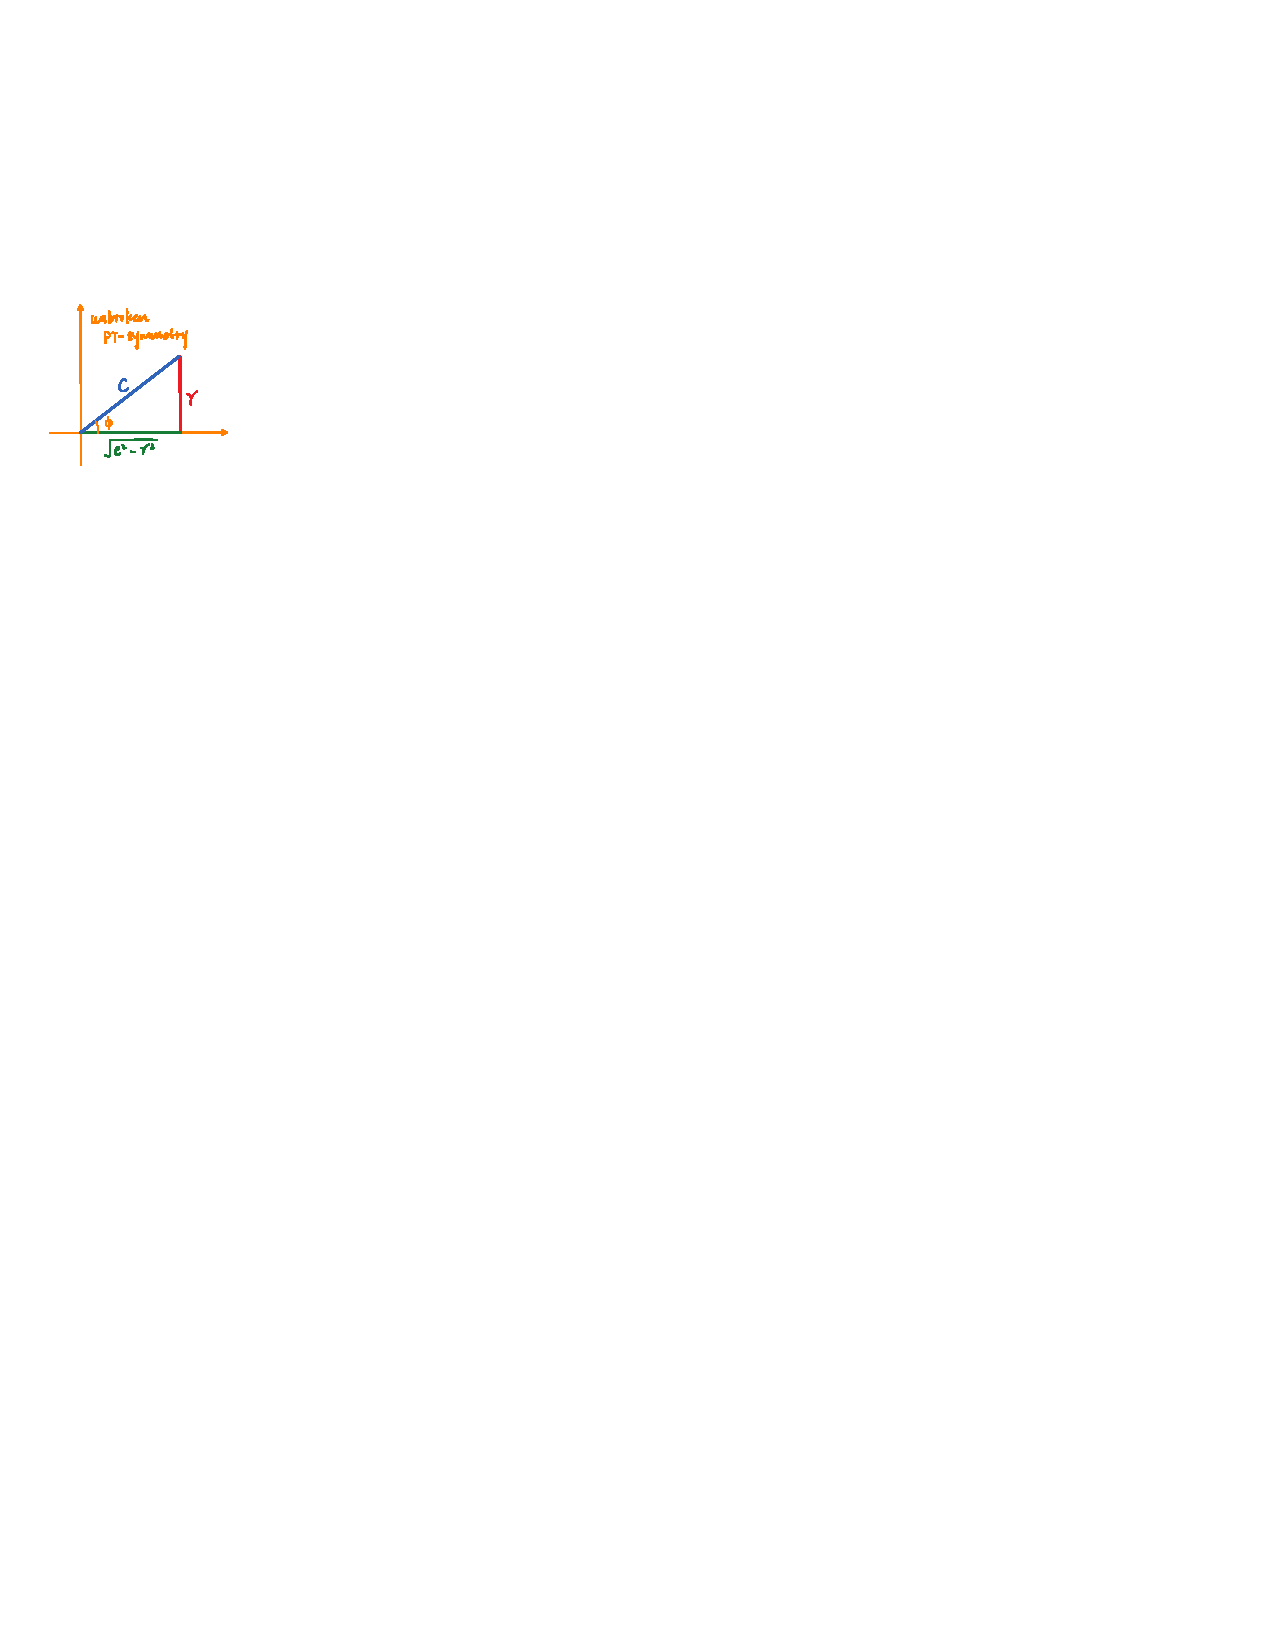
\includegraphics[scale=2.5]{2x2Unborken.pdf}
\end{center}

\hfill\break
\hfill\break
\hfill\break
Without lost of generality, we suppose that the $P$ and $T$ operators are isometries, that is, they preserve the length of the eigensolutions of the system. 

\begin{thm}
Let $n \in \N$, let $\mathcal{H} \in \text{Mat}_{n\times n}(\Complex)$ be commute with $PT$ where $P$ is a linear isometry and $T$ is an antilinear isometry. Consider the system $\mathcal{H}\psi	 = E\psi$ for some $E \in \Complex$ and $\psi \in \Complex^n$, with $\dim(\{\phi \mid \mathcal{H}\phi = E\phi\}) =1$. We have $E \in \R$ if and only if $PT \psi = \lambda \psi$ for some $\lambda \in \Complex$ with $|\lambda| = 1$.
\end{thm}
\begin{proof}
First we will show the $\Rightarrow$ direction holds. Suppose that we have $E \in \R$, here we denote $PT \psi = \mu$, then by the linearity of $P$ and the antilinearity of $T$, we have:
\begin{align*}
PT \mathcal{H}\psi = PT E\psi = E^* PT \psi = E PT \psi = E\mu \tag{1}
\end{align*}
Since $PT$ commutes with $\mathcal{H}$, then we also have:
\begin{align*}
PT \mathcal{H} \psi =\mathcal{H} PT \psi = \mathcal{H} \mu \tag{2}
\end{align*}
Hence combining (1) and (2) we get:
\begin{align*}
E\mu = \mathcal{H}\mu \tag{3}
\end{align*}
Since $PT$ is an isometry, then we get:
\begin{align*}
||\psi|| = ||\mu|| \tag{4}
\end{align*}
From (3), and since $\dim(\{ \phi \mid \mathcal{H}\phi = E\phi\}) = 1$, we get:
\begin{align*}
PT \psi = \mu = \lambda \psi  \qquad \text{for some }\lambda \in \Complex \tag{5}
\end{align*}
Combining (4) and (5), we get:
\begin{align*}
||\psi|| = ||\mu|| = ||\lambda\psi|| = |\lambda | \cdot ||\psi|| \qquad \Rightarrow \qquad |\lambda | = 1
\end{align*}
This completes the proof of the $\Rightarrow$ direction.\\
For the $\Leftarrow$ direction, we suppose that $PT\psi= \lambda \psi$ for some $\lambda \in \Complex$ with $|\lambda| = 1$. By linearity of $P$ and antilinearity of $T$, we can write:
\begin{align*}
\mathcal{H}PT\psi =  PT\mathcal{H}\psi = PT E\psi = E^* PT\psi = E^*\lambda \psi \tag{6}
\end{align*}
Since $\dim(\{ \phi \mid \mathcal{H}\phi = E\phi\}) = 1$ and $\lambda \psi \in \{ \phi \mid \mathcal{H}\phi = E\phi\}$, equation (6) forces $E^* = E$, and hence $E \in \R$. This completes the proof of the $\Leftarrow$ direction, the result of this theorem follows.
\end{proof}

\newpage
\section{Extend to a $3\times 3$ Hamiltonian}
For the $2\times 2$ Hamiltonian, we can plot its eigenvalues over the gain $\gamma$ of one of the cavity bands:\\

Parameters: $C = 2.5$, $E = 1600$. 
\begin{center}
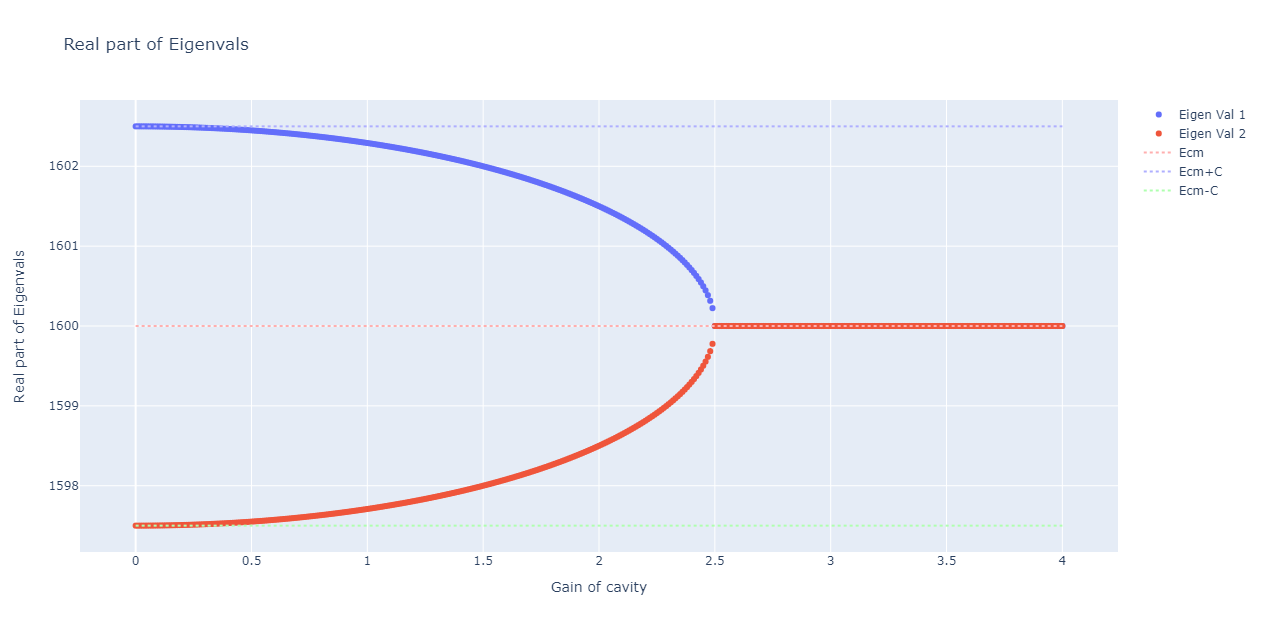
\includegraphics[scale=0.25]{2x2HamReal.png}
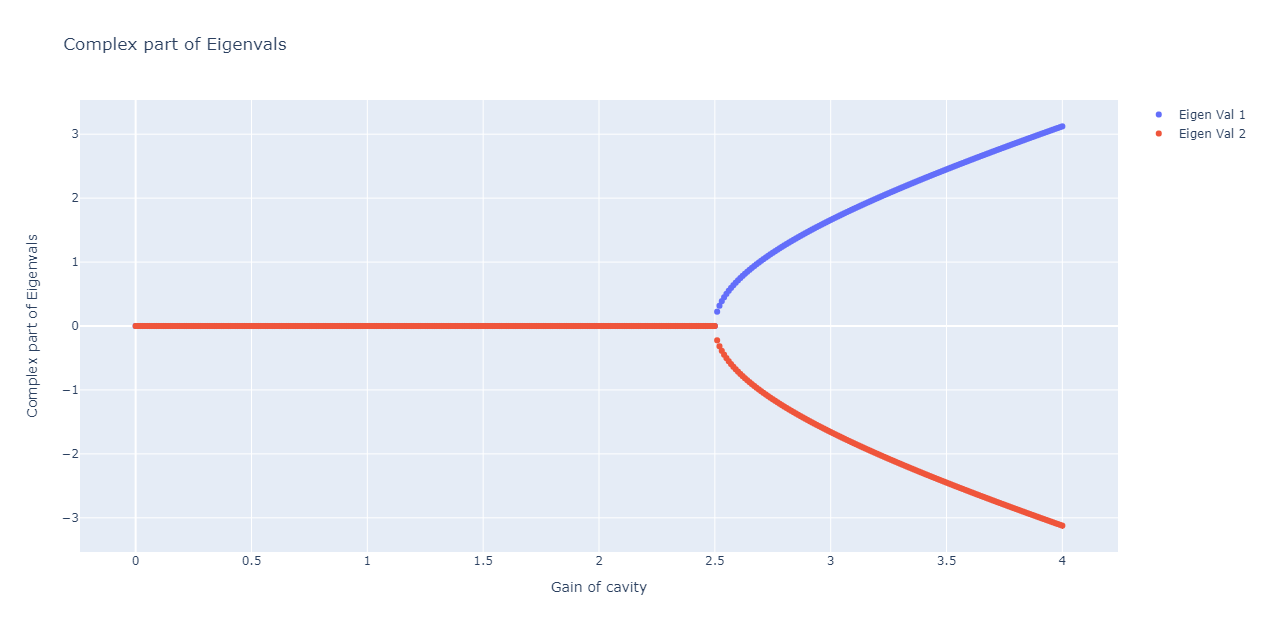
\includegraphics[scale=0.25]{2x2HamComp.png}
\end{center}

Now suppose that we add a layer of $2D$-material, such as $\text{MoSe}_2$ or any other kinds of TMDC material, on top of the coupled cavity-bands, such that the cavity bands is also coupled with an exciton. Such new system can be described by the following $3\times 3$ Hamiltonian:
\begin{align*}
\mathcal{H} = \bmat{E+i\gamma & C & \Omega/2\\
     				C & E-i\gamma & \Omega/2\\
     				\Omega/2 & \Omega/2 & Xc}
\end{align*}
This Hamiltonian is also PT-symmetric if one defines the $T$ operator to be taking complex conjugate, and the $P$ operator as the following matrix:
\begin{align*}
P = \bmat{0 & 1 & 0 \\
	      1 & 0 & 0 \\
	      0 & 0 & 1}
\end{align*}
Indeed, we have:
\begin{align*}
PT\mathcal{H}(PT)^{-1} = \mathcal{H}
\end{align*}

\hfill\break\hfill\break
In this system, we plot its eigenvalues over the gain $\gamma$ of one of the cavity bands:\\

Parameters: $C = 8$, $\Omega = 15$, $E = 1660$, $Xc = 1650$. 
\begin{center}
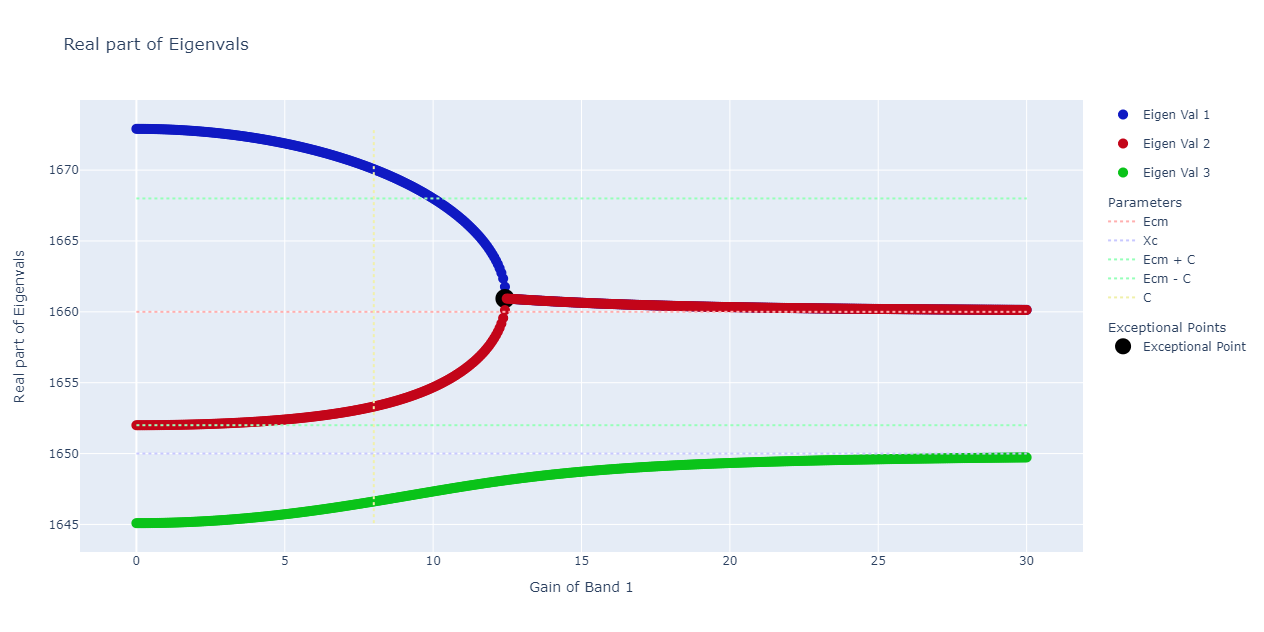
\includegraphics[scale=0.29]{081510.png}
\end{center}


\newpage
\section{Analytic results of the $3\times 3$ Hamiltonian}
Here we redefine the $3\times 3$ Hamiltonian as the following:
\begin{align*}
\mathcal{H} = \bmat{E + iG & C & R \\
	  				C & E - iG & R \\
	  				R & R & X}
\end{align*}

To simplify the results, we define the following parameters:
\begin{align*}
\kappa \coloneqq \frac{C^2-E^2-G^2+2R^2-2EX}{3}+\frac{{\left(2E+X\right)}^2}{9}
\end{align*}
\begin{align*}
\sigma \coloneqq CR^2-ER^2+\frac{E^2X+G^2X-C^2X}{2}-\frac{\left(2E+X\right)\left(-C^2+E^2+2XE+G^2-2R^2\right)}{6}+\frac{{\left(2E+X\right)}^3}{27}
\end{align*}

\hfill\break
Then the three eigenvalues of the Hamiltonian become:
\begin{align*}
\text{val}_1=\frac{2E+X}{3}+\frac{\kappa}{{\left(\sigma+\sqrt{\sigma^2-\kappa^3}\right)}^{1/3}}+{\left(\sigma+\sqrt{{\sigma}^2-{\kappa}^3}\right)}^{1/3}
\end{align*}

\begin{align*}
\text{val}_2 =
&\frac{2E+X}{3}-\frac{1}{2}\left(\frac{\kappa}{{\left(\sigma+\sqrt{{\sigma}^2-{\kappa}^3}\right)}^{1/3}}+{\left(\sigma+\sqrt{{\sigma}^2-{\kappa}^3}\right)}^{1/3}\right)-\frac{\sqrt{3}}{2}\left(\frac{\kappa}{{\left(\sigma+\sqrt{{\sigma}^2-{\kappa}^3}\right)}^{1/3}} -{\left(\sigma+\sqrt{{\sigma}^2-{\kappa}^3}\right)}^{1/3}{}\right)\mathrm{i}
\end{align*}

\begin{align*}
\text{val}_3 =
&\frac{2E+X}{3}-\frac{1}{2}\left(\frac{\kappa}{{\left(\sigma+\sqrt{{\sigma}^2-{\kappa}^3}\right)}^{1/3}}+{\left(\sigma+\sqrt{{\sigma}^2-{\kappa}^3}\right)}^{1/3}\right)+\frac{\sqrt{3}}{2}\left(\frac{\kappa}{{\left(\sigma+\sqrt{{\sigma}^2-{\kappa}^3}\right)}^{1/3}} -{\left(\sigma+\sqrt{{\sigma}^2-{\kappa}^3}\right)}^{1/3}{}\right)\mathrm{i}
\end{align*}

\hfill\break
\hfill\break
Now define:
\begin{align*}
\zeta \coloneqq {\left(\sigma+\sqrt{\sigma^2-\kappa^3}\right)}^{1/3}
\end{align*}
Then the three eigenvalues of the Hamiltonian become:


\begin{align*}
\text{val}_1=\frac{2E+X}{3}+\left(\frac{\kappa}{\zeta}+\zeta\right)
\end{align*}

\begin{align*}
\text{val}_2= \frac{2E+X}{3}
&-\frac{1}{2}\left(\frac{\kappa}{\zeta}+\zeta\right)-\frac{\sqrt{3}}{2}\left(\frac{\kappa}{\zeta}-\zeta\right)\mathrm{i} 
\end{align*}


\begin{align*}
\text{val}_3 = \frac{2E+X}{3}
&-\frac{1}{2}\left(\frac{\kappa}{\zeta}+\zeta\right)+\frac{\sqrt{3}}{2}\left(\frac{\kappa}{\zeta}-\zeta\right)\mathrm{i} 
\end{align*}

One can show that we have $val_2 = val_3$ if and only if we have:
\begin{align*}
\kappa^3 = \sigma^2 \qquad\qquad \text{or}\qquad\qquad \zeta^2 = \kappa
\end{align*}


\newpage
\section{Non-PT-symmetric system}
In reality, it is not easy to make the two-phonic bands coupled with the exciton at the same amount, so it will be more realistic if we can include some analysis on the system that has unequal $\Omega$:
\begin{align*}
\mathcal{H} = \bmat{E+i\gamma & C & \color{red}\Omega_1\color{black}/2\\
     				C & E-i\gamma & \color{blue}\Omega_2\color{black}/2\\
     				\color{red}\Omega_1\color{black}/2 & \color{blue}\Omega_2\color{black}/2 & Xc}
\end{align*}
One important thing to notice here is that this Hamiltonian is not PT-symmetric anymore, as one can check that $PT\mathcal{H} (PT)^{-1} \neq \mathcal{H}$. But the plot of the eigenvalues of this system also give us some interesting results:\\

Parameters: $C = 8$, $Xc=1650$, $\Omega_1 = 9.5$, $\Omega_2 = 10$, $E = 1657.5$.
\begin{center}
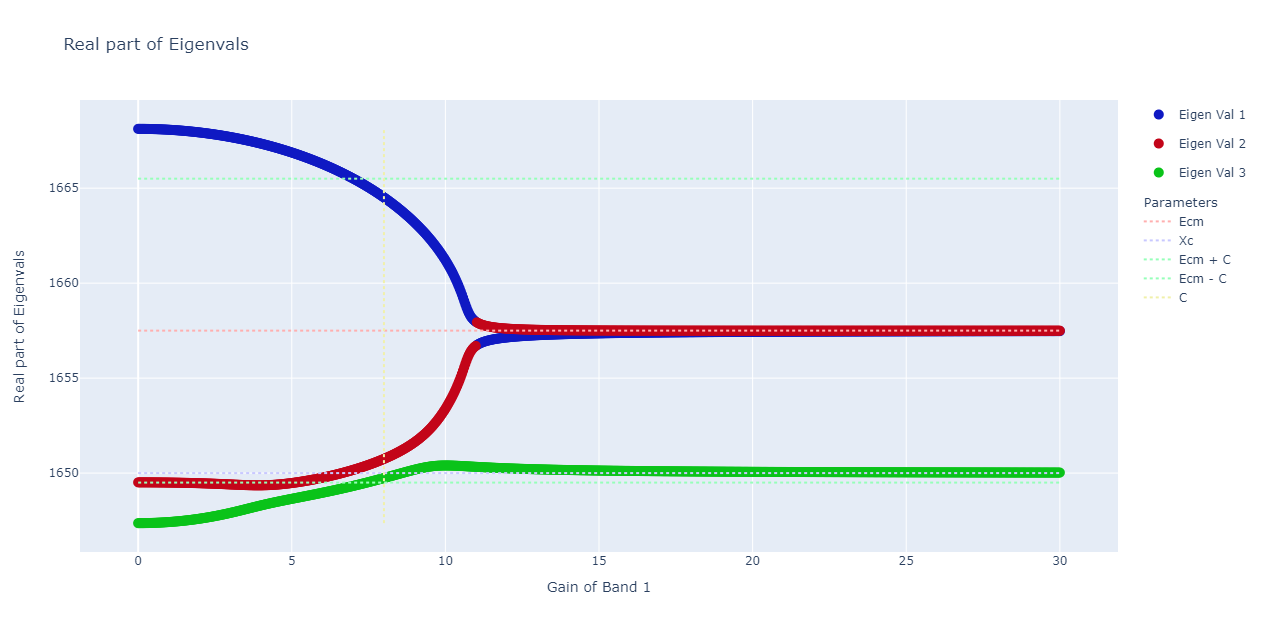
\includegraphics[scale=0.25]{DiffRabiC.png}\\
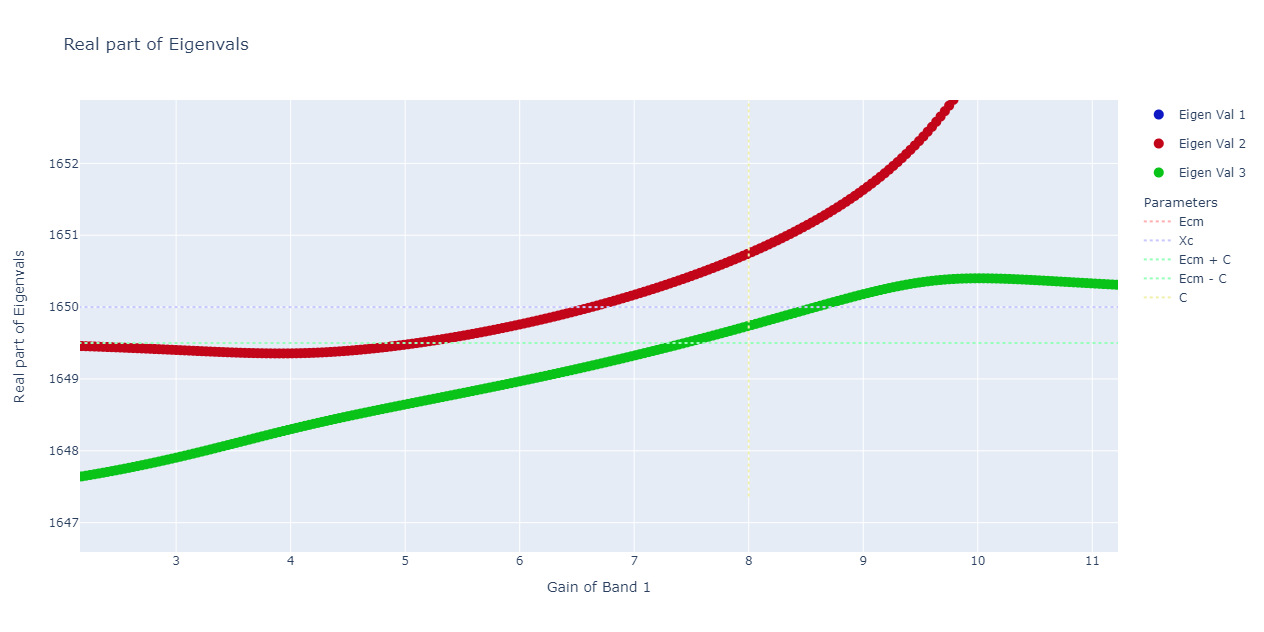
\includegraphics[scale=0.25]{ZoomedDiffRabiC.png}
\end{center}

\end{document}